\section{A Matheuristic for the \AMD}\label{Math}
\noindent
This section is devoted to present our matheuristic approach to provide good feasible solutions of the \AMD. Our motivation comes from the fact that the exact method based on the mathematical programming formulation presented in the previous section can be highly time demanding. Alternatively, the matheuristic provides good quality solution in limited computing times.\\
\noindent

Assuming that the drone has enough endurance to visit every target, the basic idea of the algorithm is to associate each target to one operation by solving a crossing postman problem with neighbors  (XPPN) (see \cite{Puerto2021}) for the targets including $orig$ and $dest$. The motivation of this approach comes from the results in \cite{Puerto2021} which show that the XPPN is easily solvable for medium-size instances provided that the neighbors are points or polygonal chains. 
In the following, we present the pseudo-code of this algorithm:



\begin{itemize} 
\item[STEP 1] (Order of visit the targets)\\
Compute the order of visit by solving the XPPN for the targets of the problem including $orig$ as the first point in the tour and $dest$ as the last one and associate each target $t\in\mathcal T$ to one operation $o\in\mathcal O$ in the given order.
\item [STEP 2] (Solution of the \AMD\space model by fixing an initial partial solution)\\
Set the values of the binary variables $u^{to}$, $v^{to}$, $\delta^{to}$ and $y^{tt'o}$ provided by the solution of STEP 1 and solve the resulting \AMD\space model to obtain a complete feasible solution.
\end{itemize}

%}

It is possible to refine the previous algorithm, by slightly modifying STEP 2. Indeed, after STEP 1, starting from the first visited target, according with the order provided by the XPPN solution, we can iteratively add the next target to the same operation, if the drone endurance allows it. In this way the number of operations can be reduced and a better initial partial solution can be provided to start STEP 2.


Figure \ref{fig:Fig7} shows the solution obtained, by means of the matheuristic, for the same example of Figure \ref{fig:Fig1}. In particular, the upper subfigure reports the solution after STEP 2 in its original form. We can observe that the solution consists in the mothership tour represented in blue and in four operations of the drone. Indeed, the drone first visits the 50\% of the target with label 4 ($u^{41}=v^{41}=1$), then flies to meet the mothership at the retrieve point $x_R^1$ and from there starts its second operation to visit a 50\% of the target with label 3 ($u^{32}=v^{32}=1$). After that, the drone flies to the retrieve point $x_R^2$, it visits another 50\% of the target with label 2 and then, from the launch point $x_L^4$ it starts its last operation to visit also another 50\% of the the target with label 1 ($u^{14}=v^{14}=1$). Then, it flies to the last retrieve point $x_R^4$ and moves to the destination point together with the mothership.
In the lower subfigure of Figure \ref{fig:Fig7} we can observe the solution obtained with the modified version of STEP 2. Differently from the upper one, the number of drone operations is equal to two. Indeed, thanks to the refinement of STEP 2, the drone endurance permits to visit the two targets with label 4 and 3 in the first operation  ($u^{41}=v^{31}=1$ and $y^{431}=1$). Similarly, the drone can also visit two targets, namely 2 and 1, in its second operation ($u^{22}=v^{12}=1$ and $y^{212}=1$).\\ 
In terms of objective function values, in this example, the refinement of STEP 2 does not provide an improved solution. Indeed, its value is equal to 888.01 without refinement and equal to 920.4 with the refinement of STEP 2. 
However, the length of the mothership tour, when STEP 2 is implemented in its original form, is equal to 189.72, while with the refinement of STEP 2 it is equal to 180.39. 
Moreover, we point out that the total time associated with the mothership tour is shorter in the solution without refinement of STEP 2. This is due to the different number of stops performed by the mothership in the two solutions. Indeed, in the solution obtained by the refinement, the number of mothership stops is 4 instead of 5 and, in some of them, the mothership waits for the drone. Summing up, in this example the refinement of STEP 2 generates a solution with a shorter tour of the mothership but with a weighted sum of the distances travelled by both, drone and mothership, that is worse than the one obtained without refinement. In general, depending on the instance and the weighting factor of the two terms in the objective function, the refinement of STEP 2 can provide better solutions. For this reason in the implementation we compared the solutions obtained with and without this refinement, and we select the best one to be provided as initial solution for the exact model.


\pgfplotsset{compat=1.15}
\usetikzlibrary{arrows}
\definecolor{ffqqqq}{rgb}{1,0,0}
\definecolor{qqqqff}{rgb}{0,0,1}
\definecolor{ffqqff}{rgb}{1,0,1}
\definecolor{xfqqff}{rgb}{0.4980392156862745,0,1}
\definecolor{ududff}{rgb}{0.30196078431372547,0.30196078431372547,1}
\definecolor{yqqqqq}{rgb}{0.5019607843137255,0,0}
\definecolor{qqwwtt}{rgb}{0,0.4,0.2}
\begin{figure}[h!]
\centering
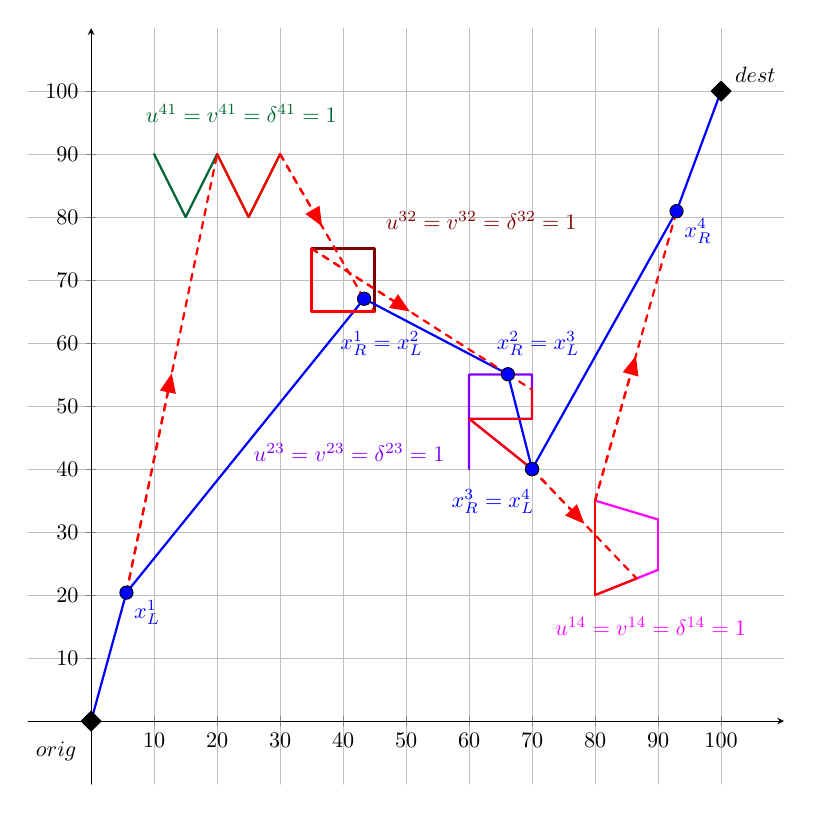
\begin{tikzpicture}[line cap=round,line join=round,>=triangle 45,x=1cm,y=1cm, scale = 0.8]
\begin{axis}[
x=0.1cm,y=0.1cm,
axis lines=middle,
ymajorgrids=true,
xmajorgrids=true,
xmin=-10,
xmax=110,
ymin=-10,
ymax=110,
xtick={0,10,...,100},
ytick={0,10,...,100},]
\clip(-49.903883687724594,-14.69149547687434) rectangle (209.13223427513805,134.7784315983007);
\draw [line width=1pt,color=qqwwtt] (10,90)-- (15,80)-- (20,90)-- (25,80)-- (30,90);
\draw [line width=1pt] (35,75)-- (35,65);
\draw [line width=1pt] (35,65)-- (45,65);
\draw [line width=1pt,color=yqqqqq] (45,65)-- (45,75);
\draw [line width=1pt,color=yqqqqq] (45,75)-- (35,75);
\draw [line width=1pt,color=xfqqff] (60,40)-- (60,55)-- (70,55)-- (70,48)-- (60,48)-- (70,40);
\draw [line width=1pt] (80,35)-- (80,20);
\draw [line width=1pt,color=ffqqff] (80,20)-- (90,24);
\draw [line width=1pt,color=ffqqff] (90,24)-- (90,32);
\draw [line width=1pt,color=ffqqff] (90,32)-- (80,35);
\draw (-10,-2) node[anchor=north west] {$\bm{orig}$};
\draw (101,105) node[anchor=north west] {$\bm{dest}$};
\draw [line width=1pt,color=qqqqff] (0,0)-- (5.6057,20.3868);
\draw [line width=1pt,color=qqqqff] (5.6057,20.3868)-- (43.33,67.04);
\draw [line width=1pt,color=qqqqff] (43.33,67.04)-- (66.16,55.06);
\draw [line width=1pt,color=qqqqff] (66.16,55.06)-- (70,40);
\draw [line width=1pt,color=qqqqff] (70,40)-- (92.93,80.94);
\draw [line width=1pt,color=qqqqff] (92.93,80.94)-- (100,100);
\draw [line width=1pt,dashed,color=ffqqqq] (5.6057,20.3868)-- (20,90);
\draw [line width=1pt,color=ffqqqq] (20,90)-- (25,80);
\draw [line width=1pt,color=ffqqqq] (25,80)-- (30,90);
\draw [line width=1pt,dashed,color=ffqqqq] (30,90)-- (43.33,67.04);
\draw [line width=1pt,dashed,color=ffqqqq] (43.33,67.04)-- (45,65);
\draw [line width=1pt,color=ffqqqq] (45,65)-- (35,65);
\draw [line width=1pt,color=ffqqqq] (35,65)-- (35,75);
\draw [line width=1pt,dashed,color=ffqqqq] (35,75)-- (66.16,55.06);
\draw [line width=1pt,dashed,color=ffqqqq] (66.16,55.06)-- (70,52.5969);
\draw [line width=1pt,color=ffqqqq] (70,52.5969)-- (70,48);
\draw [line width=1pt,color=ffqqqq] (70,48)-- (60,48);
\draw [line width=1pt,color=ffqqqq] (60,48)-- (70,40);
\draw [line width=1pt,dashed,color=ffqqqq] (70,40)-- (86.5971,22.6388);
\draw [line width=1pt,color=ffqqqq] (86.5971,22.6388)-- (80,20);
\draw [line width=1pt,color=ffqqqq] (80,20)-- (80,35);
\draw [line width=1pt,dashed,color=ffqqqq] (80,35)-- (92.93,80.94);
\draw [->,line width=1pt,dashed,color=ffqqqq] (5.6057,20.3868) -- (12.80285,55.1934);
\draw [->,line width=1pt,dashed,color=ffqqqq] (30,90) -- (36.665,78.52);
\draw [->,line width=1pt,dashed,color=ffqqqq] (35,75) -- (50.58,65.03);
\draw [->,line width=1pt,dashed,color=ffqqqq] (70,40) -- (78.29855,31.3194);
\draw [->,line width=1pt,dashed,color=ffqqqq] (80,35) -- (86.465,57.97);
\draw [color=qqwwtt](7.45897147725058,99.14529141107357) node[anchor=north west] {$\bm{u^{41}=v^{41}=\delta^{41}=1}$};
\draw [color=yqqqqq](45.53179129265427,82.1934233173285) node[anchor=north west] {$\bm{u^{32}=v^{32}=\delta^{32}=1}$};
\draw [color=xfqqff](24.55585724578162,45.26562117671086) node[anchor=north west] {$\bm{u^{23}=v^{23}=\delta^{23}=1}$};
\draw [color=ffqqff](72.43552748014484,17.620603501925224) node[anchor=north west] {$\bm{u^{14}=v^{14}=\delta^{14}=1}$};
\begin{scriptsize}
\draw [fill=black] (0,0) ++(-4.5pt,0 pt) -- ++(4.5pt,4.5pt)--++(4.5pt,-4.5pt)--++(-4.5pt,-4.5pt)--++(-4.5pt,4.5pt);
\draw [fill=black] (100,100) ++(-4.5pt,0 pt) -- ++(4.5pt,4.5pt)--++(4.5pt,-4.5pt)--++(-4.5pt,-4.5pt)--++(-4.5pt,4.5pt);
\draw [fill=ududff] (70,40) circle (3pt);
\draw [color=qqqqff] (56,38) node[anchor=north west]{\bm{$x_R^3=x_L^4$}};
\draw [fill=qqqqff] (5.6057,20.3868) circle (3pt);
\draw [color=qqqqff] (5.6057,20.3868) node[anchor=north west]{$\bm{x_L^1}$};
\draw [fill=qqqqff] (43.33,67.04) circle (3pt);
\draw [color=qqqqff] (38.33,63.04) node[anchor=north west]{$\bm{x_R^1=x_L^2}$};
\draw [fill=qqqqff] (66.16,55.06) circle (3pt);
\draw [color=qqqqff] (63.16,63.04) node[anchor=north west]{$\bm{x_R^2=x_L^3}$};
\draw [fill=qqqqff] (70,40) circle (3pt);
\draw [fill=qqqqff] (92.93,80.94) circle (3pt);
\draw [color=qqqqff] (92.93,80.94) node[anchor=north west]{$\bm{x_R^4}$};
\end{scriptsize}
\end{axis}
\end{tikzpicture}

\definecolor{ffqqqq}{rgb}{1,0,0}
\definecolor{qqqqff}{rgb}{0,0,1}
\definecolor{wwttqq}{rgb}{0.4,0.2,0}
\definecolor{qqwwtt}{rgb}{0,0.4,0.2}
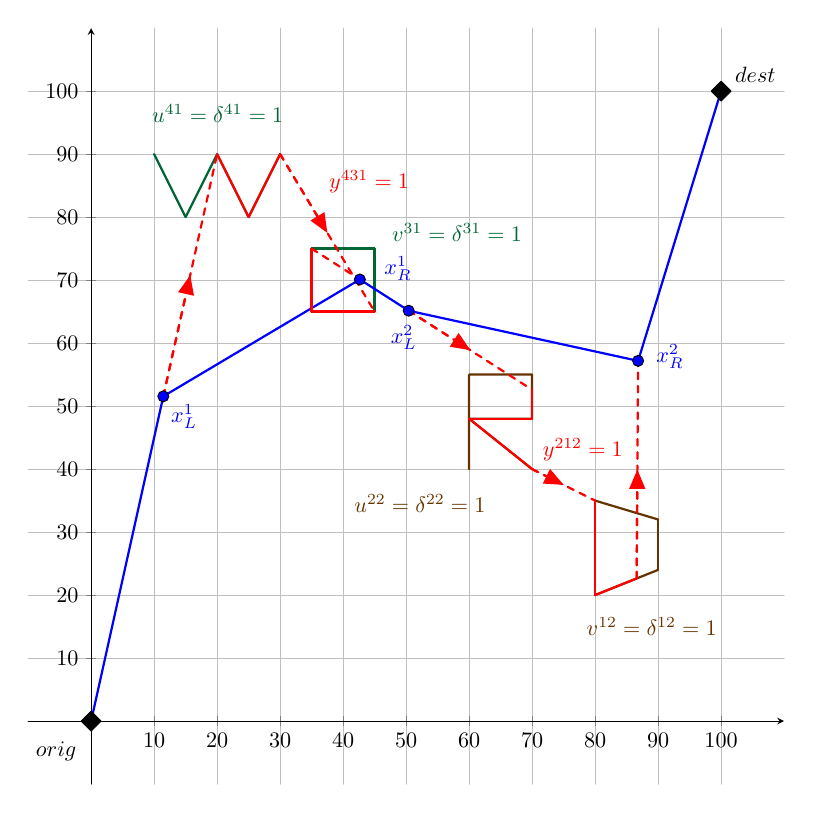
\begin{tikzpicture}[line cap=round,line join=round,>=triangle 45,x=1cm,y=1cm, scale = 0.8]
\begin{axis}[
x=0.1cm,y=0.1cm,
axis lines=middle,
ymajorgrids=true,
xmajorgrids=true,
xmin=-10,
xmax=110,
ymin=-10,
ymax=110,
xtick={0,10,...,100},
ytick={0,10,...,100},]
%\clip(-51.87275387205345,-19.48294075374569) rectangle (135.90040875888684,125.1089370909846);
\draw [line width=1pt,color=qqwwtt] (10,90)-- (15,80)-- (20,90)-- (25,80)-- (30,90);
\draw [line width=1pt] (35,75)-- (35,65);
\draw [line width=1pt] (35,65)-- (45,65);
\draw [line width=1pt,color=qqwwtt] (45,65)-- (45,75);
\draw [line width=1pt,color=qqwwtt] (45,75)-- (35,75);
\draw [line width=1pt,color=wwttqq] (60,40)-- (60,55)-- (70,55)-- (70,48)-- (60,48)-- (70,40);
\draw [line width=1pt] (80,35)-- (80,20);
\draw [line width=1pt,color=wwttqq] (80,20)-- (90,24);
\draw [line width=1pt,color=wwttqq] (90,24)-- (90,32);
\draw [line width=1pt,color=wwttqq] (90,32)-- (80,35);
\draw (-10,-2) node[anchor=north west] {$\bm{orig}$};
\draw (101,105) node[anchor=north west] {$\bm{dest}$};
\draw [color=qqwwtt](8.45897147725058,99.14529141107357) node[anchor=north west] {\bm{$u^{41}=\delta^{41}=1$}};
\draw [color=qqwwtt](46.53179129265427,80.1934233173285) node[anchor=north west] {\bm{$v^{31}=\delta^{31}=1$}};
\draw [color=wwttqq](40.55585724578162,37.26562117671086) node[anchor=north west] {\bm{$u^{22}=\delta^{22}=1$}};
\draw [color=wwttqq](77.43552748014484,17.620603501925224) node[anchor=north west] {\bm{$v^{12}=\delta^{12}=1$}};
\draw [line width=1pt,color=qqqqff] (0,0)-- (11.46,51.55);
\draw [line width=1pt,color=qqqqff] (11.46,51.55)-- (42.66,70.1);
\draw [line width=1pt,color=qqqqff] (42.66,70.1)-- (50.41,65.14);
\draw [line width=1pt,color=qqqqff] (50.41,65.14)-- (86.83,57.18);
\draw [line width=1pt,color=qqqqff] (86.83,57.18)-- (100,100);
\draw [line width=1pt,dashed,color=ffqqqq] (11.46,51.55)-- (20,90);
\draw [line width=1pt,color=ffqqqq] (20,90)-- (25,80);
\draw [line width=1pt,color=ffqqqq] (25,80)-- (30,90);
\draw [line width=1pt,dashed,color=ffqqqq] (30,90)-- (45,65);
\draw [line width=1pt,color=ffqqqq] (45,65)-- (35,65);
\draw [line width=1pt,color=ffqqqq] (35,65)-- (35,75);
\draw [line width=1pt,dashed,color=ffqqqq] (35,75)-- (42.66,70.1);
% \draw [line width=1pt,color=ffqqqq] (42.66,70.1)-- (11.46,51.55);
\draw [line width=1pt,dashed,color=ffqqqq] (50.41,65.14)-- (70,52.6);
\draw [line width=1pt,color=ffqqqq] (70,52.6)-- (70,48);
\draw [line width=1pt,color=ffqqqq] (70,48)-- (60,48);
\draw [line width=1pt,color=ffqqqq] (60,48)-- (70,40);
\draw [line width=1pt,dashed,color=ffqqqq] (70,40)-- (80,35);
\draw [line width=1pt,color=ffqqqq] (80,35)-- (80,20);
\draw [line width=1pt,color=ffqqqq] (80,20)-- (86.6,22.64);
\draw [line width=1pt,dashed,color=ffqqqq] (86.6,22.64)-- (86.83,57.18);
\draw [->,line width=1pt,dashed,color=ffqqqq] (11.46,51.55) -- (15.73,70.775);
\draw [->,line width=1pt,dashed,color=ffqqqq] (50.41,65.14) -- (60.205,58.87);
\draw [->,line width=1pt,dashed,color=ffqqqq] (86.5971,22.6388) -- (86.715,39.91);
\draw [->,line width=1pt,dashed,color=ffqqqq] (30,90) -- (37.5,77.5);
\draw [->,line width=1pt,dashed,color=ffqqqq] (70,40) -- (75,37.5);
\draw [color=ffqqqq](36.54173818934138,88.70826534025115) node[anchor=north west] {\bm{$y^{431}=1$}};
\draw [color=ffqqqq](70.47421968887281,46.158736277919324) node[anchor=north west] {\bm{$y^{212}=1$}};
\begin{scriptsize}
\draw [fill=black] (0,0) ++(-4.5pt,0 pt) -- ++(4.5pt,4.5pt)--++(4.5pt,-4.5pt)--++(-4.5pt,-4.5pt)--++(-4.5pt,4.5pt);
\draw [fill=black] (100,100) ++(-4.5pt,0 pt) -- ++(4.5pt,4.5pt)--++(4.5pt,-4.5pt)--++(-4.5pt,-4.5pt)--++(-4.5pt,4.5pt);
\draw [fill=qqqqff] (11.46,51.55) circle (2.5pt);
\draw [color=qqqqff](11.46,51.55) node[anchor=north west] {\bm{$x_L^1$}};
\draw [fill=qqqqff] (42.66,70.1) circle (2.5pt);
\draw [color=qqqqff] (45.33,75.04) node[anchor=north west]{$\bm{x_R^1}$};
\draw [fill=qqqqff] (50.41,65.14) circle (2.5pt);
\draw [color=qqqqff] (46.33,64.04) node[anchor=north west]{$\bm{x_L^2}$};
\draw [fill=qqqqff] (86.83,57.18) circle (2.5pt);
\draw [color=qqqqff] (88.5,61.04) node[anchor=north west]{$\bm{x_R^2}$};
\end{scriptsize}
\end{axis}
\end{tikzpicture}
\caption{Solution provided by the matheuristic.}
\label{fig:Fig7}
\end{figure}